\documentclass[aspectratio=169]{beamer}

% Theme and color scheme
\usetheme{Madrid}
\usecolortheme{default}
\setbeamertemplate{navigation symbols}{}
\setbeamertemplate{footline}[frame number]

% Packages
\usepackage{amsmath}
\usepackage{amssymb}
\usepackage{bm}
\usepackage{graphicx}
\usepackage{booktabs}
\usepackage{multirow}
\usepackage{subcaption}
\usepackage{algorithm}
\usepackage{algorithmic}
\graphicspath{{figures}}

% Color definitions
\definecolor{tumaroon}{RGB}{157,34,53}
\setbeamercolor{palette primary}{bg=tumaroon,fg=white}
\setbeamercolor{palette secondary}{bg=tumaroon!80,fg=white}
\setbeamercolor{palette tertiary}{bg=tumaroon!60,fg=white}
\setbeamercolor{palette quaternary}{bg=tumaroon!40,fg=black}
\setbeamercolor{structure}{fg=tumaroon}
\setbeamercolor{section in toc}{fg=tumaroon}
\setbeamercolor{frametitle}{bg=tumaroon,fg=white}

%%%%%%%%%%%%%%%%%%%%%%%%%%%%%%%%%%%%%%%%%%%%%%%%%%%%%
\title[GNSS-Denied Geophysical Navigation]{Navigation in GNSS-Denied Environments\\
Using MEMS-Grade Sensors and Geophysical Anomalies:\\
A Particle Filter Approach}

\author[Brodovsky \& Dames]{James Brodovsky \and Philip Dames}
\institute[Temple University]{Department of Mechanical Engineering\\Temple University}
\date{14 April 2026}

%%%%%%%%%%%%%%%%%%%%%%%%%%%%%%%%%%%%%%%%%%%%%%%%%%%%%
\begin{document}

\begin{frame}
    \titlepage
\end{frame}

%-----------------------------------------------------
\begin{frame}{Outline}
    \tableofcontents
\end{frame}

%%%%%%%%%%%%%%%%%%%%%%%%%%%%%%%%%%%%%%%%%%%%%%%%%%%%%
\section{Motivation}

\begin{frame}{GNSS Is Ubiquitous---and Vulnerable}
    \begin{columns}
        \begin{column}{0.55\textwidth}
            \textbf{GNSS limitations:}
            \begin{itemize}
                \item Relies on weak RF signals from orbit
                \item \textbf{Denial:} urban canyons, indoors, underground, underwater
                \item \textbf{Jamming:} electronic warfare can block signals over wide areas
                \item \textbf{Spoofing:} false signals inject position errors silently
            \end{itemize}
            \vspace{0.4em}
            \textbf{Consequences:}
            \begin{itemize}
                \item Inertial Navigation Systems (INS) drift rapidly without GNSS corrections
                \item Critical for aviation, maritime, autonomous vehicles, military
            \end{itemize}
        \end{column}
        \begin{column}{0.42\textwidth}
            \begin{block}{Rapid INS Drift}
                \small
                Without corrections, MEMS-grade IMUs accumulate \textbf{kilometers of error} over minutes of flight/drive time.
            \end{block}
            \vspace{0.5em}
            \begin{alertblock}{Alt-PNT is Needed}
                \small
                Alternative Positioning, Navigation, and Timing (Alt-PNT) that does \textbf{not} rely on external RF signals.
            \end{alertblock}
        \end{column}
    \end{columns}
\end{frame}

%-----------------------------------------------------
\begin{frame}{Geophysical Navigation: A Passive Alternative}
    \begin{columns}
        \begin{column}{0.55\textwidth}
            \textbf{Key idea:} Earth's gravity and magnetic fields have spatial structure.
            \vspace{0.5em}
            \begin{itemize}
                \item \textbf{Gravity anomaly:} deviation of local gravity from theoretical model---mapped globally at $\sim$1.8\,km resolution (IGPP)
                \item \textbf{Magnetic anomaly:} deviation of local field from IGRF model---mapped at $\sim$5.6\,km resolution (WDMAM)
                \item Compare \emph{sensed} values to \emph{map} values $\rightarrow$ position estimate via map-matching
                \item Entirely passive, no RF emissions
            \end{itemize}
            \vspace{0.5em}
            \textbf{Prior art:} demonstrated in aerospace/maritime with \emph{navigation-grade} sensors (RLG/FOG IMUs, dedicated gravimeters and magnetometers)
        \end{column}
        \begin{column}{0.42\textwidth}
            \begin{exampleblock}{Open Question}
                \small
                Does geophysical navigation remain viable with \textbf{MEMS-grade sensors} (\$10--\$1,000) and publicly available, lower-resolution maps?
            \end{exampleblock}
            \vspace{0.5em}
            \begin{block}{Why MEMS?}
                \small
                Smartphones, drones, small autonomous vehicles---the platforms most exposed to GNSS denial are the ones that cannot carry high-grade sensors.
            \end{block}
        \end{column}
    \end{columns}
\end{frame}

%-----------------------------------------------------
\begin{frame}{Prior Work and This Contribution}
    \begin{columns}
        \begin{column}{0.52\textwidth}
            \textbf{Prior work (Brodovsky \& Dames, ION ITM 2026):}
            \begin{itemize}
                \item Integrated gravity \& magnetic anomaly into an \textbf{Unscented Kalman Filter} (UKF) INS
                \item MEMS-grade sensors + open-source maps
                \item Demonstrated feasibility; limited by Gaussian assumption
            \end{itemize}
            \vspace{0.5em}
            \textbf{Problem with UKF in map-matching:}
            \begin{itemize}
                \item Anomaly map may produce \emph{multimodal} posteriors (same reading, multiple locations)
                \item UKF collapses to single Gaussian---can diverge
            \end{itemize}
        \end{column}
        \begin{column}{0.45\textwidth}
            \begin{alertblock}{This Work}
                Replace UKF with a \textbf{Rao-Blackwellized Particle Filter} (RBPF):
                \begin{itemize}
                    \item Particles represent non-Gaussian, multimodal position hypotheses
                    \item Kalman filter per particle for linear states
                    \item Enables efficient representation of complex posteriors
                \end{itemize}
            \end{alertblock}
            \vspace{0.3em}
            \small
            First application of RBPF geophysical navigation to the MEMS-grade sensor regime.
        \end{column}
    \end{columns}
\end{frame}

%%%%%%%%%%%%%%%%%%%%%%%%%%%%%%%%%%%%%%%%%%%%%%%%%%%%%
\section{Methodology}

\begin{frame}{Dataset and Experimental Setup}
    \begin{columns}
        \begin{column}{0.55\textwidth}
            \textbf{MEMS-Nav Dataset:}
            \begin{itemize}
                \item Smartphone-grade sensors via \emph{Sensor Logger} app
                \item 21 trajectories, mostly highway driving
                \item Duration: 30 min -- several hours
                \item Distance: tens to hundreds of km
                \item Sensors: IMU (accel + gyro), GNSS, magnetometer, barometer
            \end{itemize}
            \vspace{0.5em}
            \textbf{Geophysical Maps:}
            \begin{itemize}
                \item Gravity: IGPP free-air anomaly ($\sim$1.8\,km resolution)
                \item Magnetic: WDMAM ($\sim$5.6\,km resolution)
                \item Interpolated via GMT bilinear interpolation
            \end{itemize}
        \end{column}
        \begin{column}{0.42\textwidth}
            \begin{block}{Controlled Comparison}
                \small
                Identical dataset, degradation scenarios, and maps as prior UKF work.\\[0.5em]
                Only the \textbf{filter architecture} changes (RBPF vs.\ UKF).
            \end{block}
            \vspace{0.5em}
            \begin{block}{Three Test Configurations}
                \small
                \begin{enumerate}
                    \item Gravity anomaly aiding only
                    \item Magnetic anomaly aiding only
                    \item Combined gravity + magnetic
                \end{enumerate}
                \vspace{0.2em}
                Plus two baselines: RBPF (no geo) and UKF (no geo)
            \end{block}
        \end{column}
    \end{columns}
\end{frame}
%-----------------------------------------------------
\begin{frame}{Dataset Map}
    \centering
    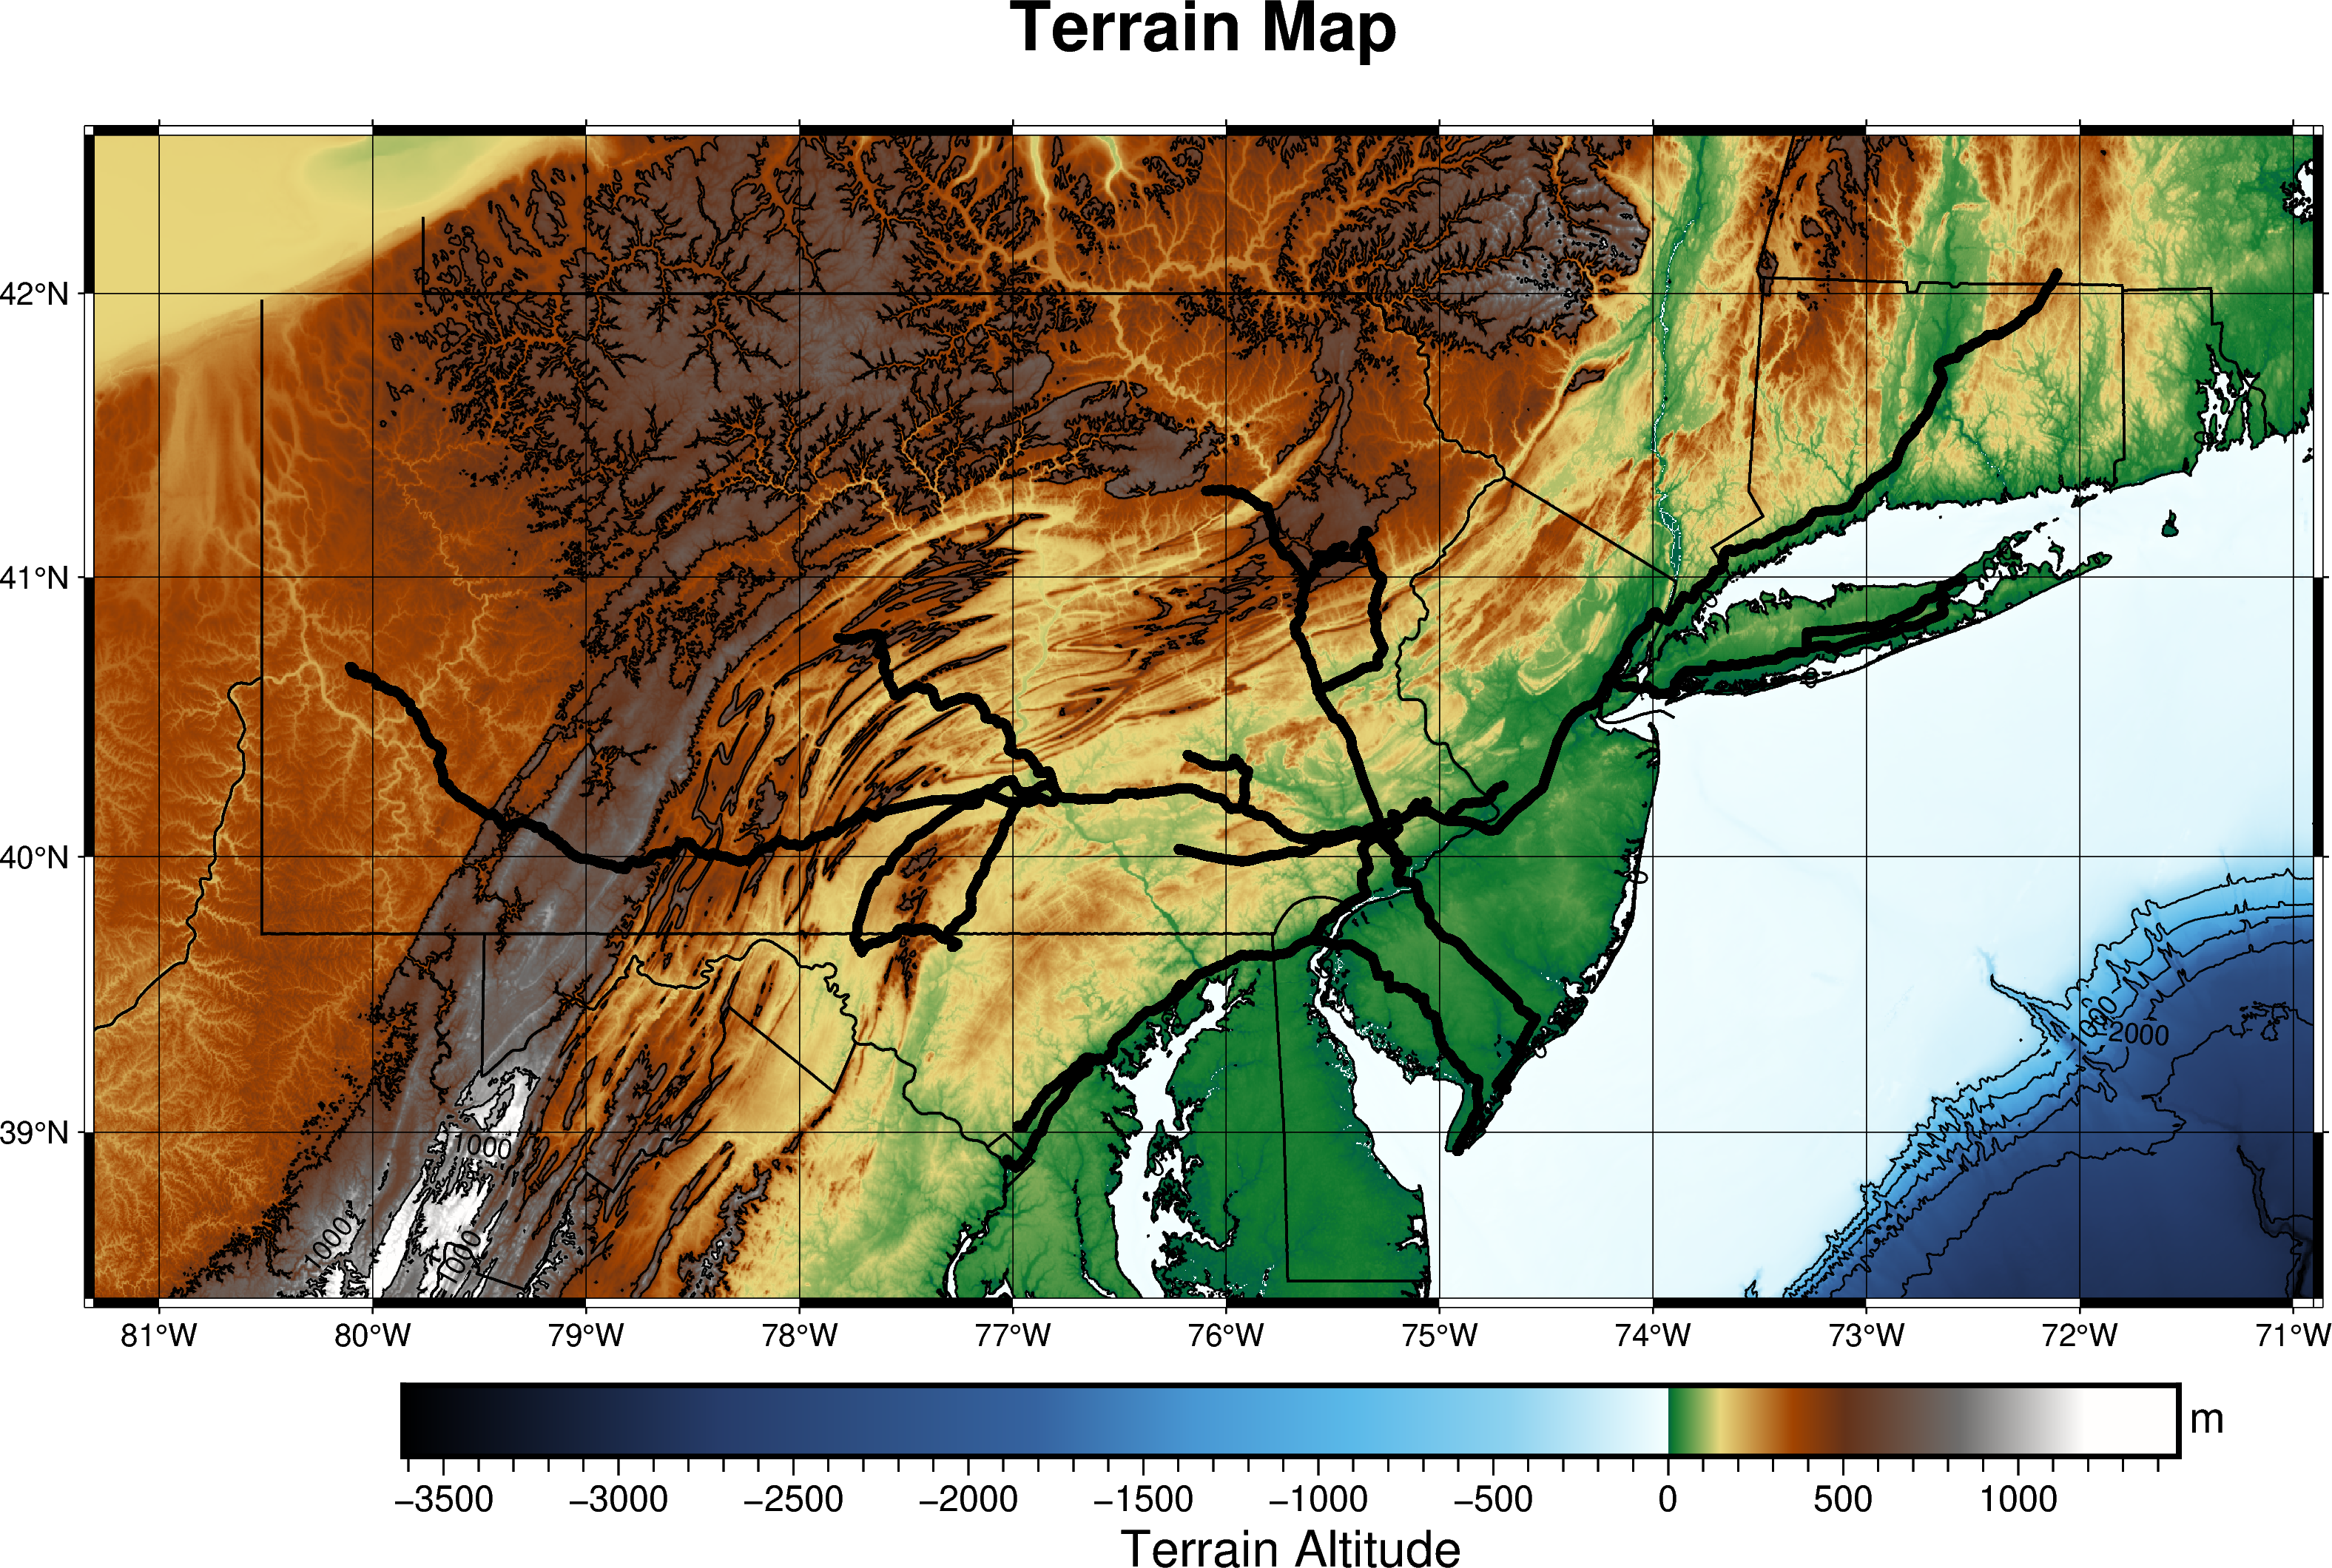
\includegraphics[width=.75\textwidth]{figures/terrain_map.png}

\end{frame}
%-----------------------------------------------------
\begin{frame}{Gravity Anomaly Map}
    \centering
    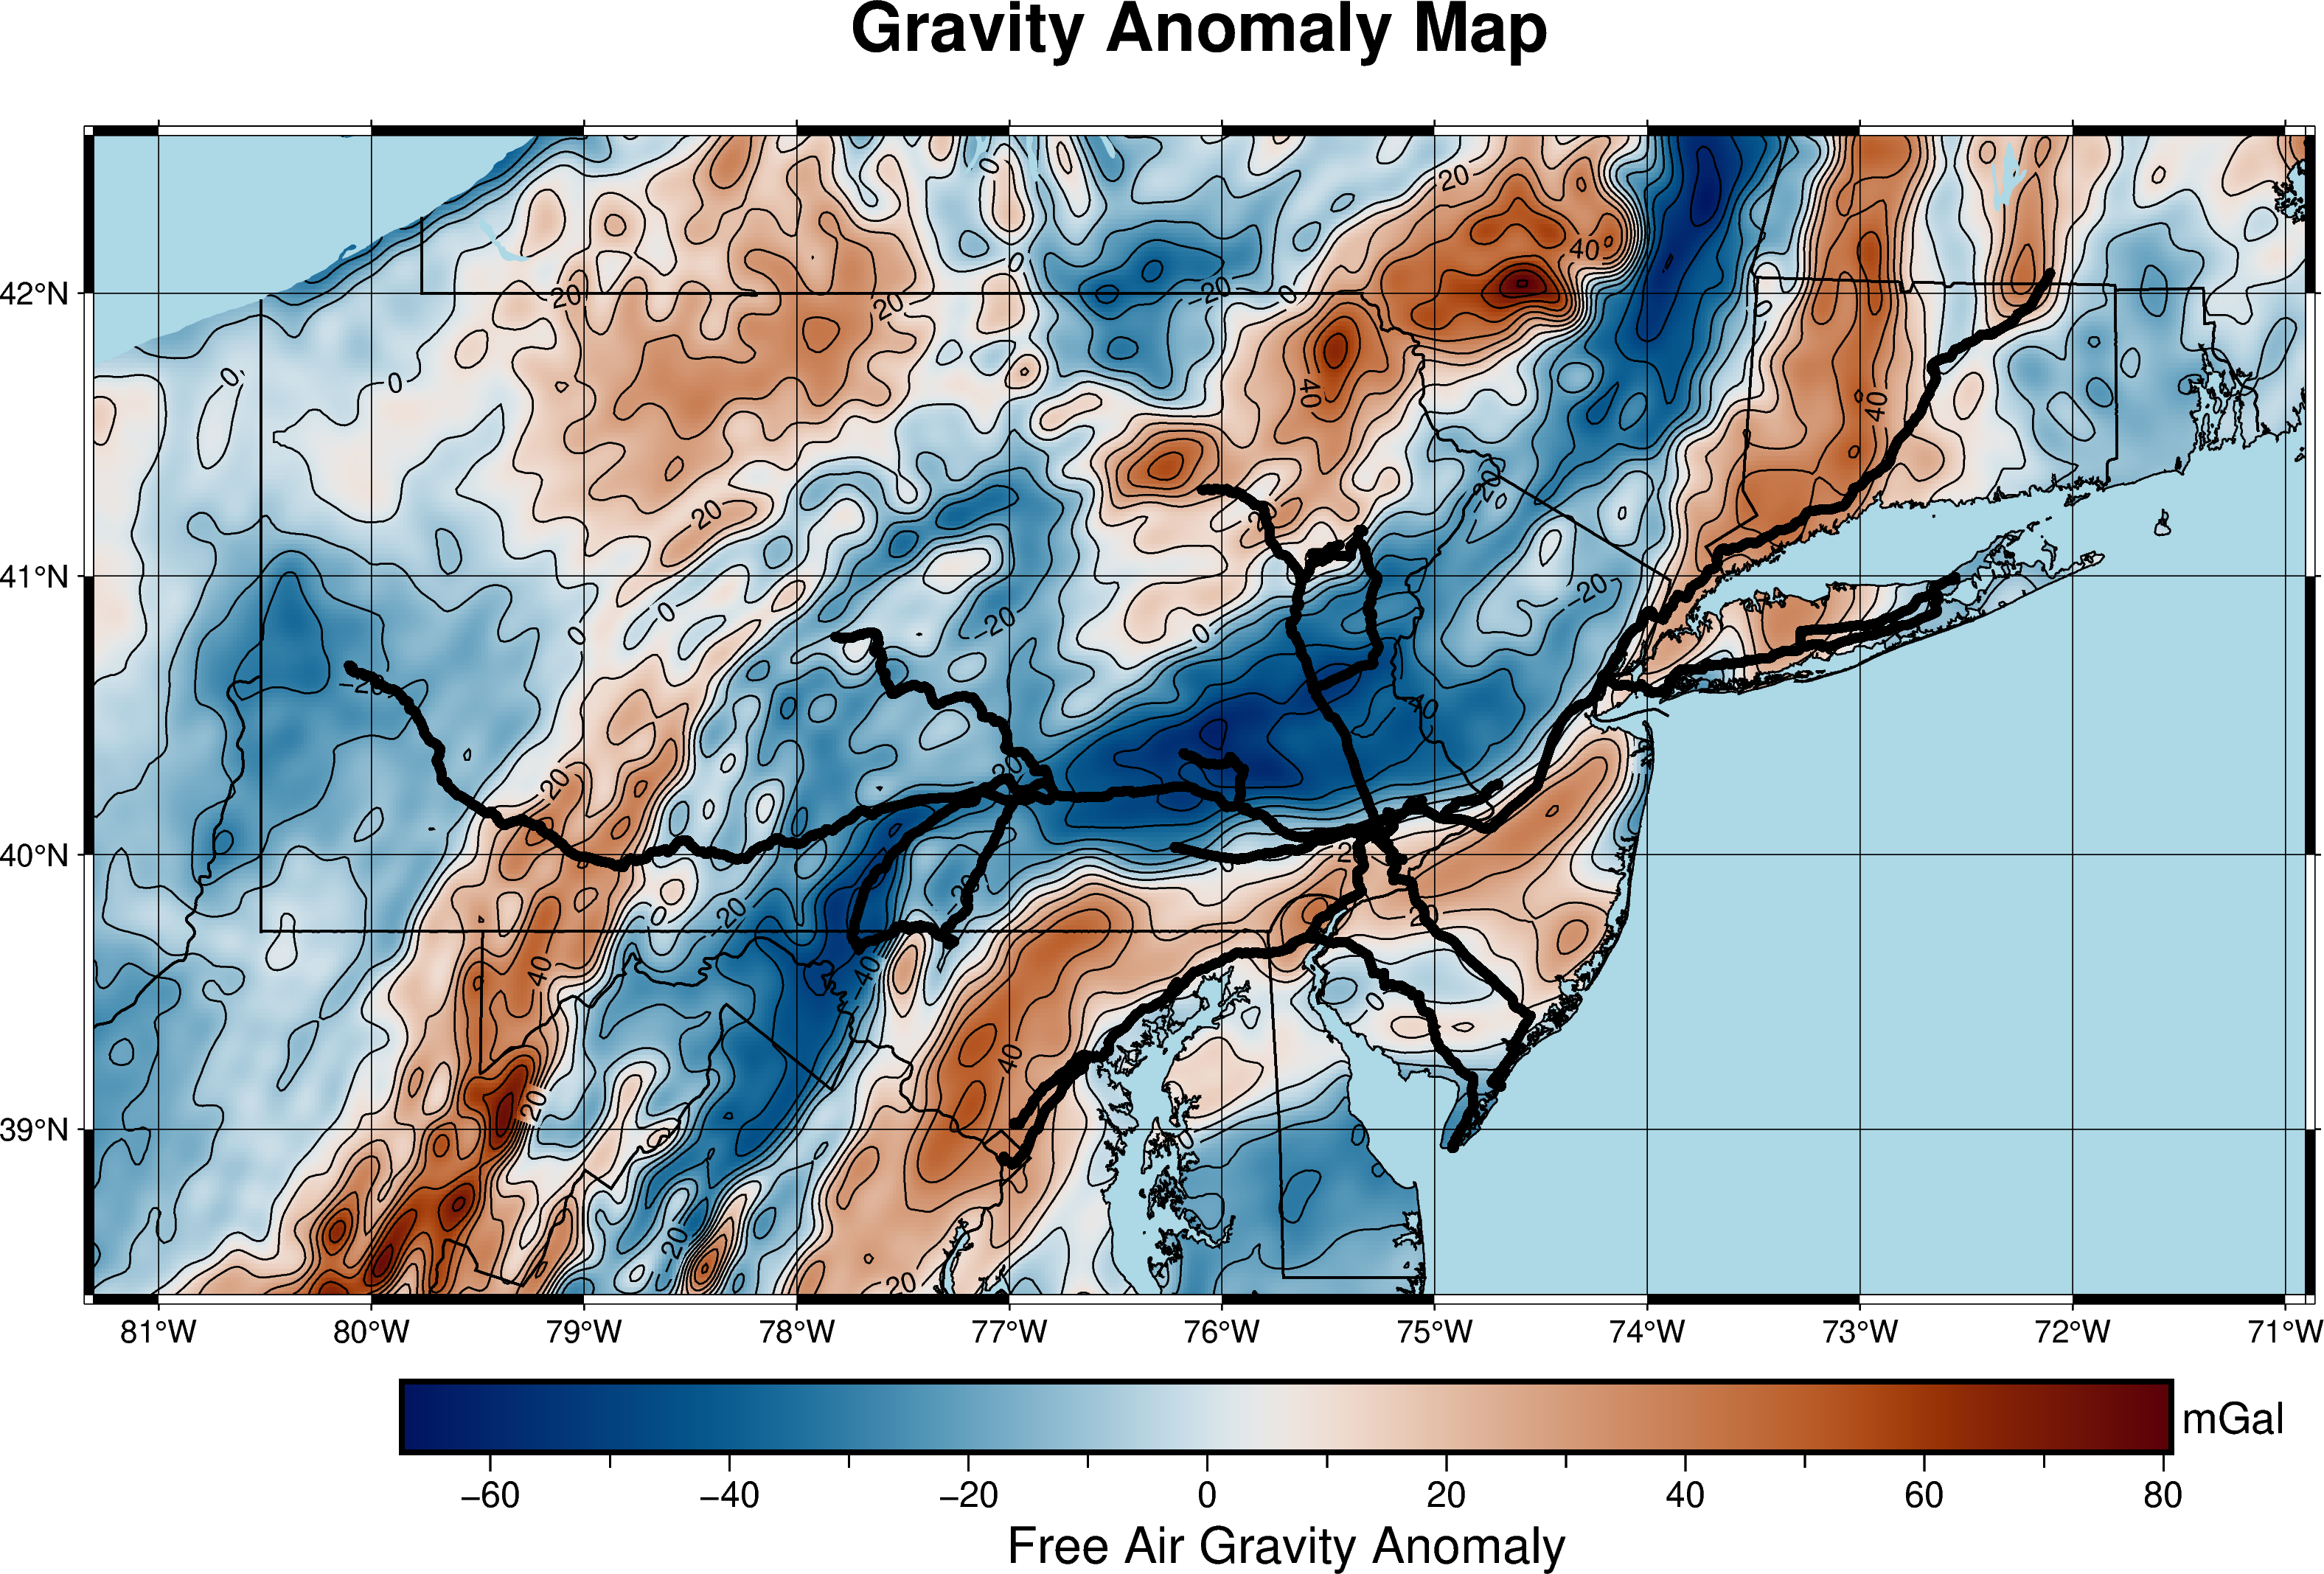
\includegraphics[width=.75\textwidth]{figures/gravity_map.png}
\end{frame}
%-----------------------------------------------------
\begin{frame}{Magnetic Anomaly Map}
    \centering
    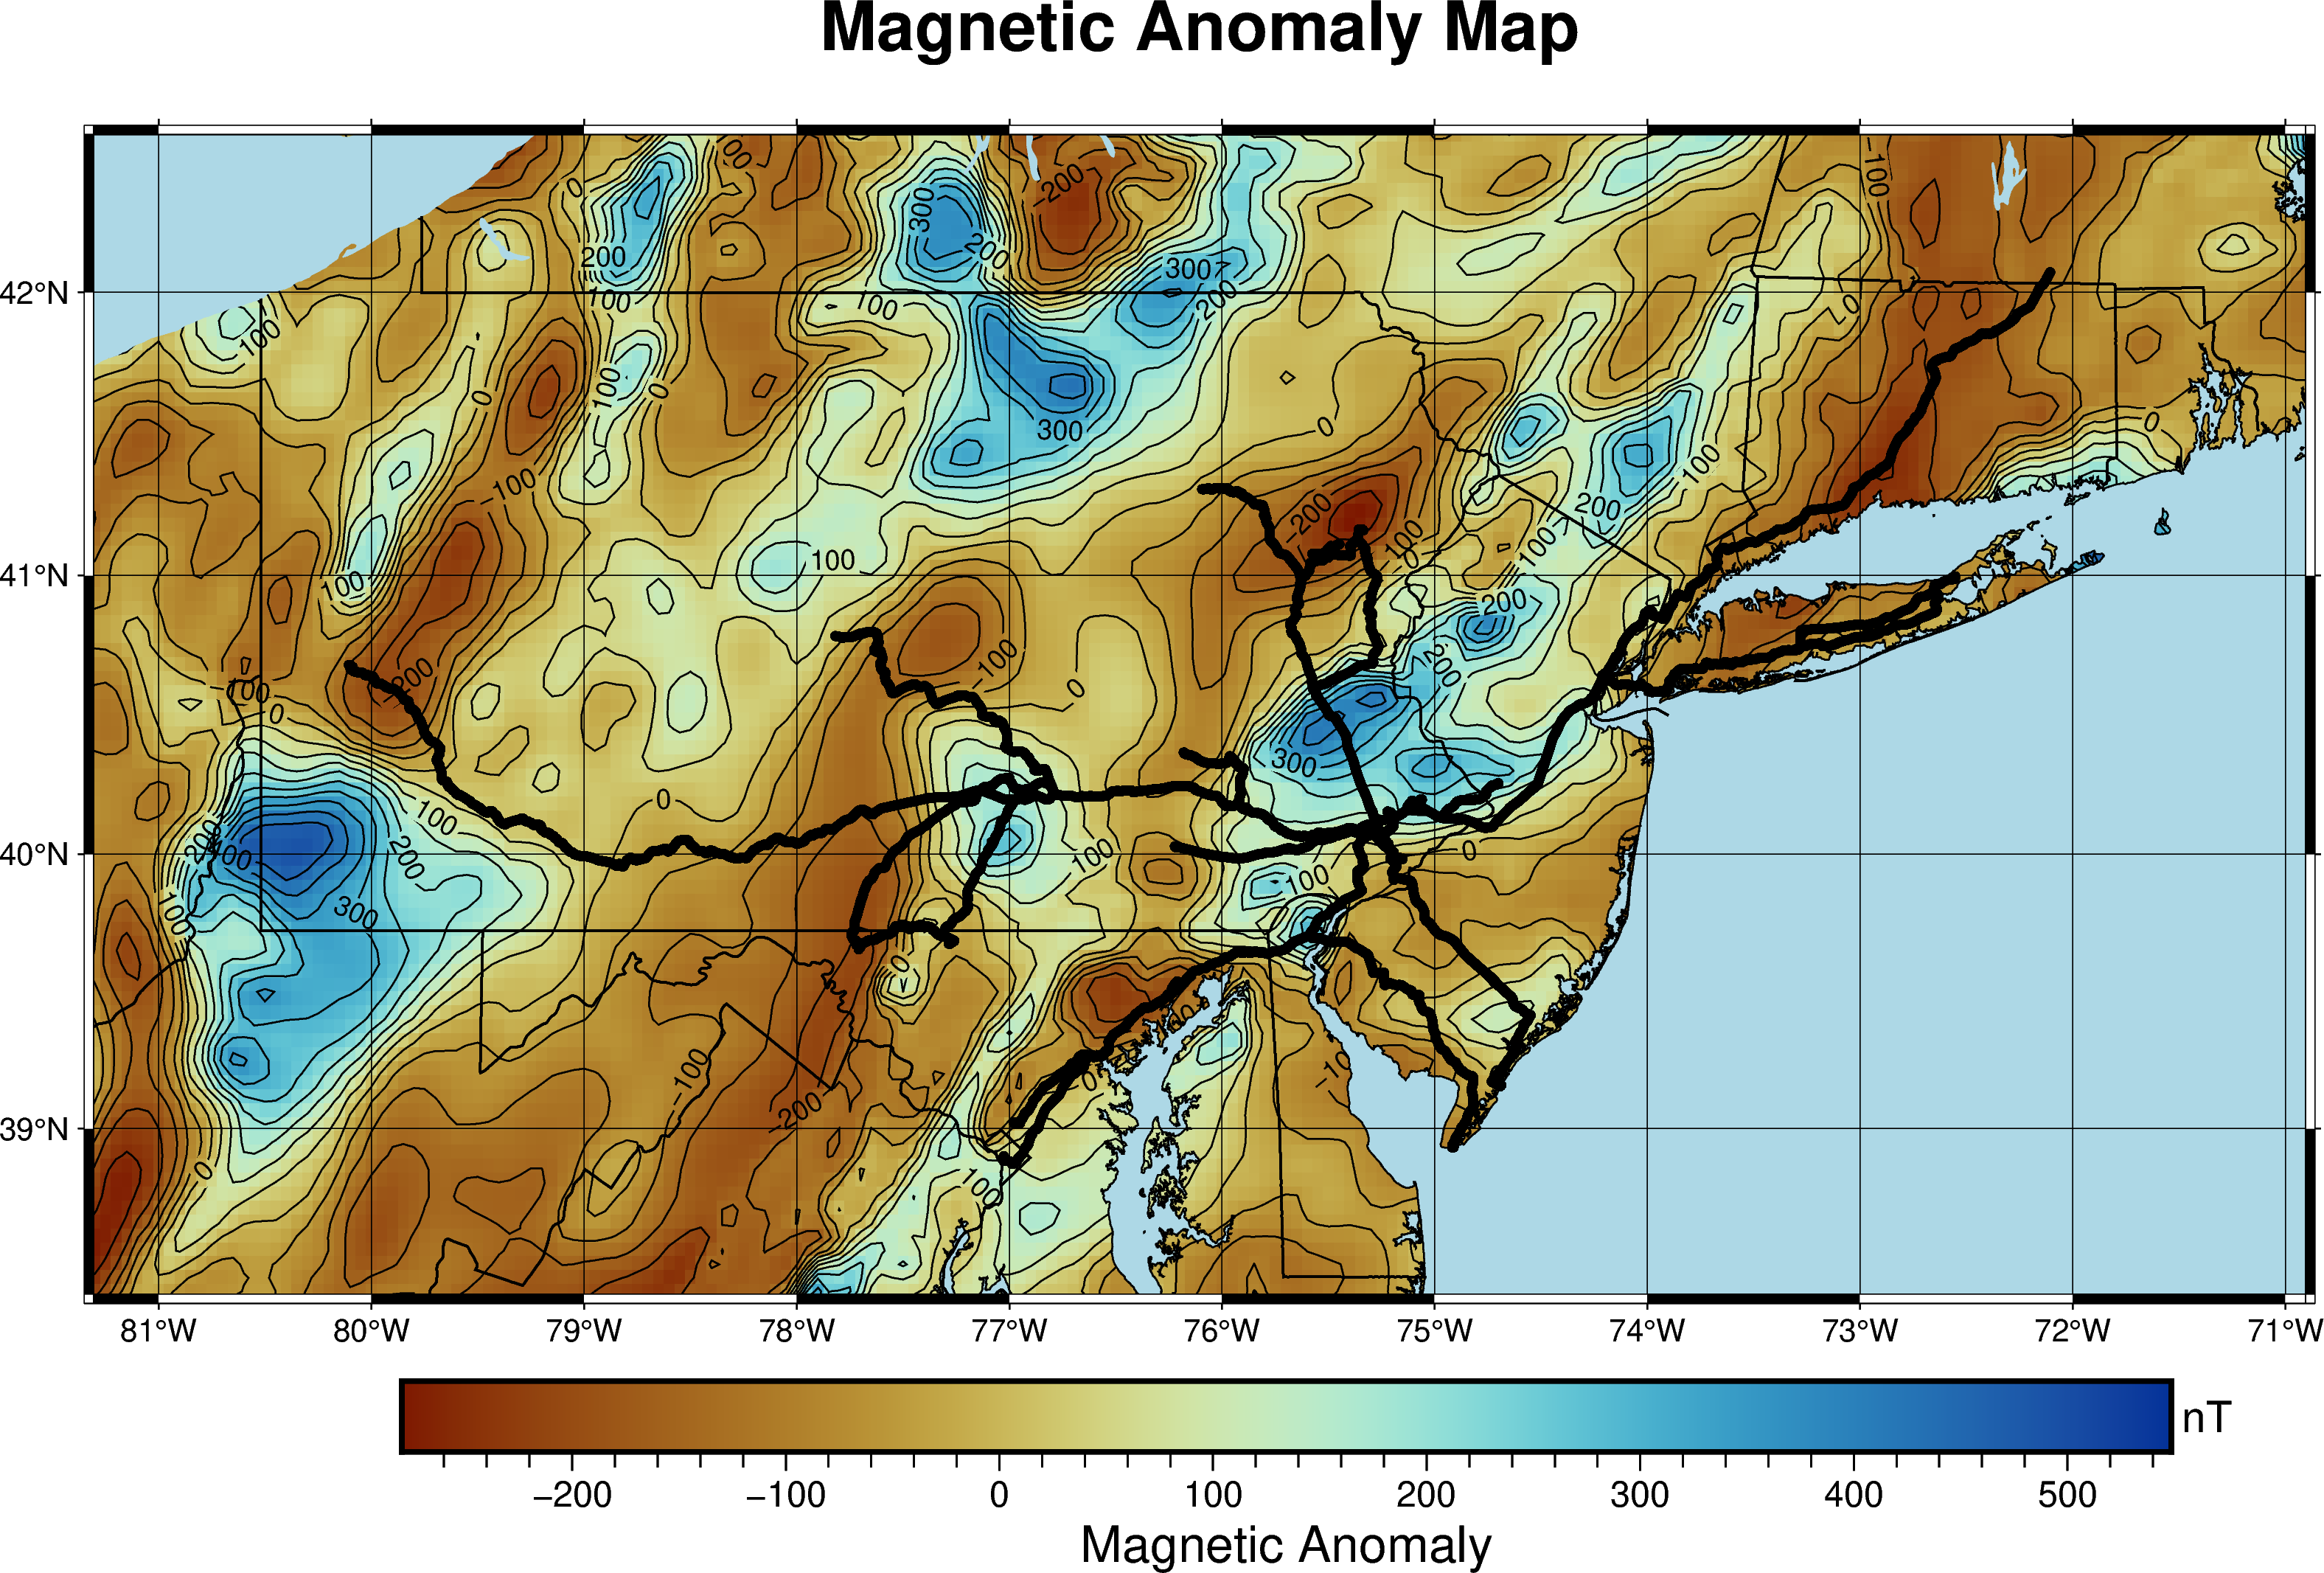
\includegraphics[width=.75\textwidth]{figures/magnetic_map.png}
\end{frame}
%-----------------------------------------------------
\begin{frame}{GNSS Degradation Model}
    \begin{columns}
        \begin{column}{0.55\textwidth}
            \textbf{Simulating realistic GNSS degradation:}
            \begin{itemize}
                \item Not simple white noise---uses \textbf{first-order autoregressive (AR(1))} error injection
                \item \textbf{Position errors:} $\rho_\text{pos} = 0.99$, $\sigma_\text{pos} = 5$\,m (slowly drifting bias)
                \item \textbf{Velocity errors:} $\rho_\text{vel} = 0.95$, $\sigma_\text{vel} = 5$\,m/s
                \item Covariance \textbf{inflated $\times 15$}: forces filter to distrust GNSS
            \end{itemize}
            \vspace{0.5em}
            \textbf{Represents:}
            \begin{itemize}
                \item Urban canyons, multipath
                \item Moderate jamming conditions
                \item Receiver reporting degraded accuracy
            \end{itemize}
        \end{column}
        \begin{column}{0.42\textwidth}
            \begin{alertblock}{Why AR(1)?}
                \small
                Real GNSS errors under multipath or jamming are \textbf{temporally correlated}, not i.i.d.\\[0.4em]
                AR(1) creates slowly wandering biases that are more challenging for the filter than white noise.
            \end{alertblock}
            \vspace{0.5em}
            \begin{block}{Same Degradation Applied to All}
                \small
                Identical parameters for both baseline and geophysically-aided runs $\Rightarrow$ controlled comparison.
            \end{block}
        \end{column}
    \end{columns}
\end{frame}

%-----------------------------------------------------
\begin{frame}{Rao-Blackwellized Particle Filter Architecture}
    \begin{columns}
        \begin{column}{0.52\textwidth}
            \textbf{Key idea---state partitioning:}
            \[
            \mathbf{x}_t = \begin{bmatrix} \underbrace{\mathbf{x}^n_t}_{\text{nonlinear}} \\ \underbrace{\mathbf{x}^l_t}_{\text{linear}} \end{bmatrix}
            \]

            \medskip
            \textbf{Nonlinear states} (particles):
            \[
            \mathbf{x}^n = \begin{bmatrix} L \\ \lambda \end{bmatrix} \quad \text{(lat, lon)}
            \]
            Particles explicitly represent multimodal position hypotheses.
            \textbf{Linear states} (Kalman filter per particle):
            \[
            \mathbf{x}^l = [h,\, v_n,\, v_e,\, v_d,\, \phi,\, \theta,\, \psi,\, \mathbf{b}_a,\, \mathbf{b}_g,\, b_\text{geo}]^\top
            \]
            14--15 states (alt, vel, attitude, IMU biases, geo bias)
        \end{column}
        \begin{column}{0.45\textwidth}
            \begin{exampleblock}{Why This Works}
                \small
                Map-matching is \textbf{highly nonlinear} in (lat, lon): same anomaly reading can match many map locations.\\[0.4em]
                Altitude, velocity, attitude, and biases are approximately \textbf{linear given position}---handled exactly by KF.\\[0.4em]
                Result: far fewer particles needed vs.\ full 16-D particle filter.
            \end{exampleblock}
        \end{column}
    \end{columns}
\end{frame}

%-----------------------------------------------------
\begin{frame}{RBPF: Prediction, Update, and Resampling}
    \begin{columns}
        \begin{column}{0.48\textwidth}
            \textbf{Prediction (each particle):}
            \begin{itemize}
                \item Propagate position via strapdown equations
                \item KF propagates linear states (velocity, attitude, biases)
            \end{itemize}

            \vspace{0.5em}
            \textbf{Measurement update (geophysical):}
            \[
            \hat{z}^{(i)} = \underbrace{M(\mathbf{x}^{n,(i)})}_{\text{map lookup}} + \underbrace{\mathbf{H}\,\mathbf{x}^{l,(i)}}_{\text{geo bias}}
            \]
            \[
            w^{(i)} \propto w^{(i)}_\text{prev} \cdot \mathcal{N}\!\left(\nu^{(i)};\, 0,\, \mathbf{S}^{(i)}\right)
            \]
            Each particle's KF also updates its linear states.
        \end{column}
        \begin{column}{0.48\textwidth}
            \textbf{Resampling:}
            \begin{itemize}
                \item Monitor effective sample size:
                \[
                N_\text{eff} = \frac{1}{\sum_i (\tilde{w}^{(i)})^2}
                \]
                \item When $N_\text{eff} < N_\text{thresh}$: \textbf{systematic resampling}
                \item Eliminates low-weight particles; duplicates high-weight ones
            \end{itemize}

            \vspace{0.4em}
            \textbf{State estimate:}
            \[
            \hat{\mathbf{x}}_t = \sum_i \tilde{w}^{(i)}_t\, \mathbf{x}^{(i)}_t
            \]
            Weighted mean across all particles.
        \end{column}
    \end{columns}
\end{frame}

%-----------------------------------------------------
\begin{frame}{Geophysical Measurement Model}
    \begin{columns}
        \begin{column}{0.55\textwidth}
            \textbf{Measurement model:}
            \[
            z_\text{geo} = M(L, \lambda) + b_\text{geo} + \nu_\text{geo}
            \]
            \begin{itemize}
                \item $M(L,\lambda)$: bilinear map interpolation at particle hypothesis
                \item $b_\text{geo}$: slowly varying sensor bias (estimated by KF)
                \item $\nu_\text{geo}$: Gaussian measurement noise
            \end{itemize}

            \vspace{0.5em}
            \textbf{Anomaly residuals} (from MEMS-Nav dataset):

            \begin{table}
                \small
                \begin{tabular}{lcc}
                    \toprule
                    Type & Mean & Std.\ Dev. \\
                    \midrule
                    Gravity & 5.97\,mGal & 48.93\,mGal \\
                    Magnetic & 40,364\,nT & 41,303\,nT \\
                    \bottomrule
                \end{tabular}
            \end{table}
        \end{column}
        \begin{column}{0.42\textwidth}
            \begin{block}{Processing Pipeline}
                \small
                \begin{enumerate}
                    \item Subtract theoretical model from sensor reading $\rightarrow$ anomaly residual
                    \item Compare residual to anomaly map value at each particle's (lat, lon)
                    \item Update particle weight based on how well they agree
                \end{enumerate}
            \end{block}
            \vspace{0.4em}
            \begin{block}{Both Sources}
                \small
                Gravity and magnetic anomalies are processed \textbf{independently}, each with its own bias state and noise parameters.
            \end{block}
        \end{column}
    \end{columns}
\end{frame}

%%%%%%%%%%%%%%%%%%%%%%%%%%%%%%%%%%%%%%%%%%%%%%%%%%%%%
\section{Results}

\begin{frame}{Results Overview: 21 Trajectories}
    \begin{columns}
        \begin{column}{0.50\textwidth}
            \textbf{RBPF (geo-aided) vs.\ RBPF baseline:}

            \vspace{0.3em}
            \begin{table}
                \small
                \begin{tabular}{lcc}
                    \toprule
                    Aiding & Mean RMSE $\Delta$ & Median \\
                    \midrule
                    Gravity    & $-1{,}565$\,km & $-1{,}476$\,km \\
                    Magnetic   & $-1{,}565$\,km & $-1{,}475$\,km \\
                    Combined   & $-1{,}566$\,km & $-1{,}476$\,km \\
                    \bottomrule
                \end{tabular}
            \end{table}

            \vspace{0.4em}
            \begin{itemize}
                \item \textbf{All 21 trajectories} show improvement vs.\ RBPF baseline
                \item Confirms: geophysical aiding, not filter architecture, drives the gain
                \item GNSS-only RBPF drifts into the thousands of km with low-quality GNSS
            \end{itemize}
        \end{column}
        \begin{column}{0.47\textwidth}
            \textbf{RBPF (geo-aided) vs.\ UKF baseline:}

            \vspace{0.3em}
            \begin{table}
                \small
                \begin{tabular}{lcc}
                    \toprule
                    Aiding & Mean RMSE $\Delta$ & Median \\
                    \midrule
                    Gravity    & $-234$\,m  & $-1{,}177$\,m \\
                    Magnetic   & $-520$\,m  & $-496$\,m \\
                    Combined   & $-1{,}395$\,m & $-659$\,m \\
                    \bottomrule
                \end{tabular}
            \end{table}

            \vspace{0.4em}
            \begin{itemize}
                \item More modest gains vs.\ UKF (0.2--1.4\,km mean RMSE)
                \item UKF degrades deterministically; RBPF has stochastic drift
                \item Combined aiding shows best RBPF advantage
            \end{itemize}
        \end{column}
    \end{columns}
\end{frame}

%-----------------------------------------------------
\begin{frame}{Example: Strong Performance}
    \begin{figure}[b]
        \centering
        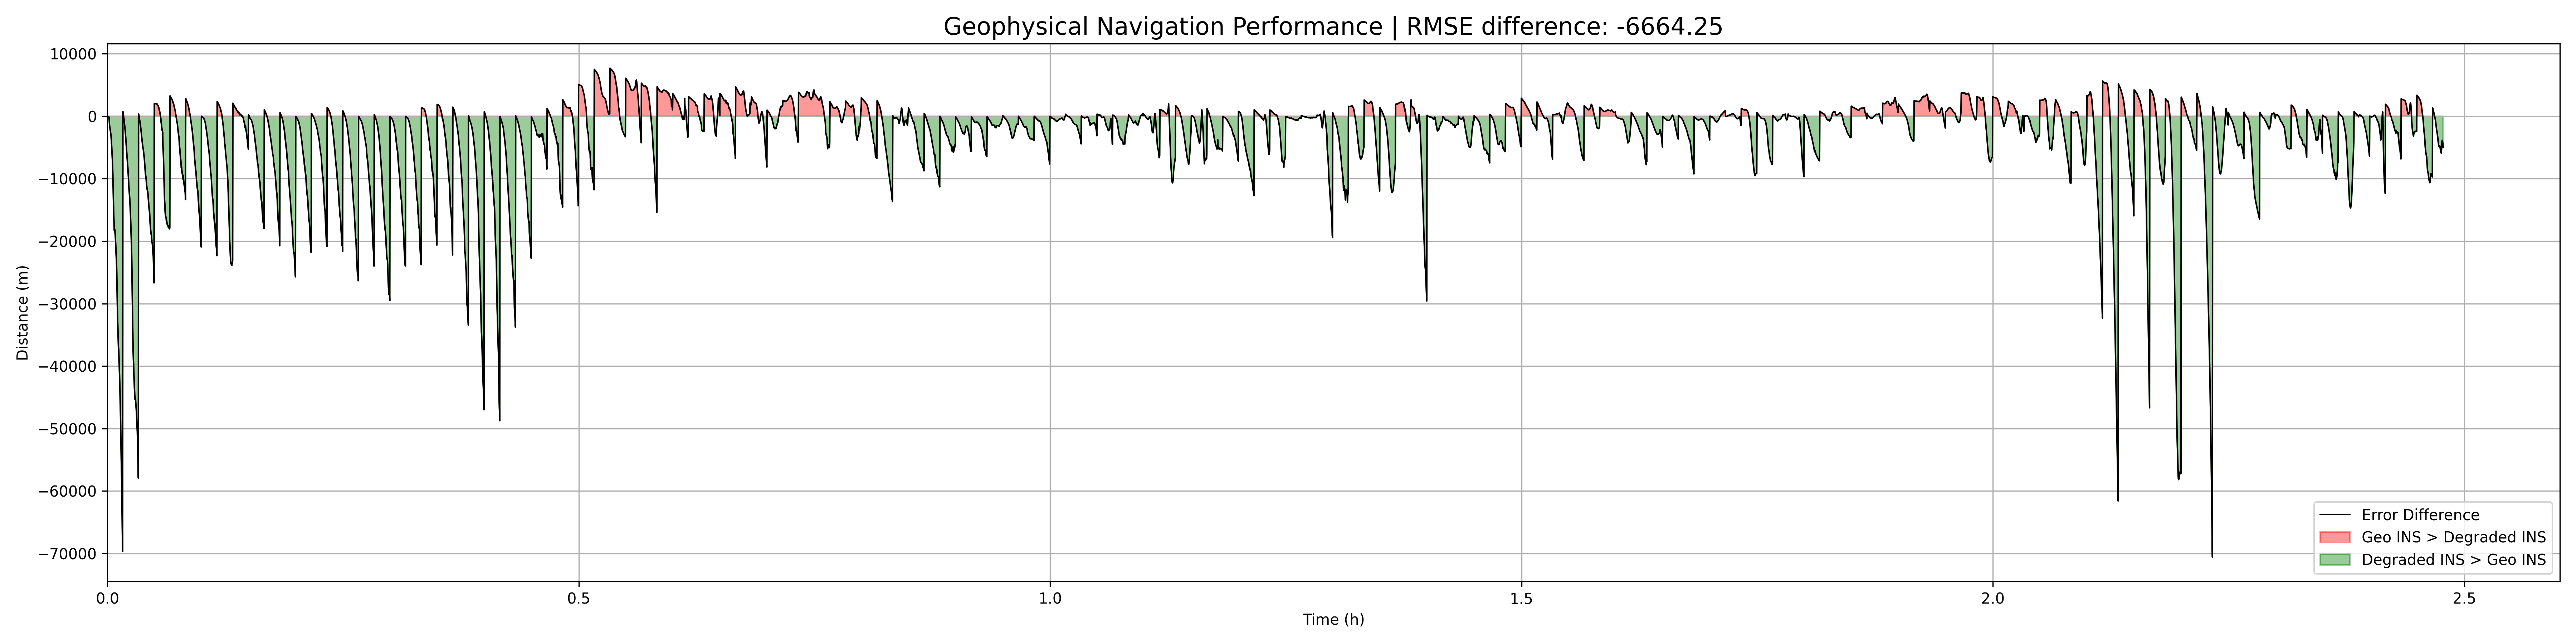
\includegraphics[width=\textwidth]{figures/good/2023-08-06_14-48-05_mag.png}
        \caption{Geo-RBPF with Magnetic aiding vs INS; 6664\,m RMSE improvement over INS baseline.}
    \end{figure}
\end{frame}
%-----------------------------------------------------
\begin{frame}{Example: Strong Performance}
\begin{figure}[b]
    \centering
    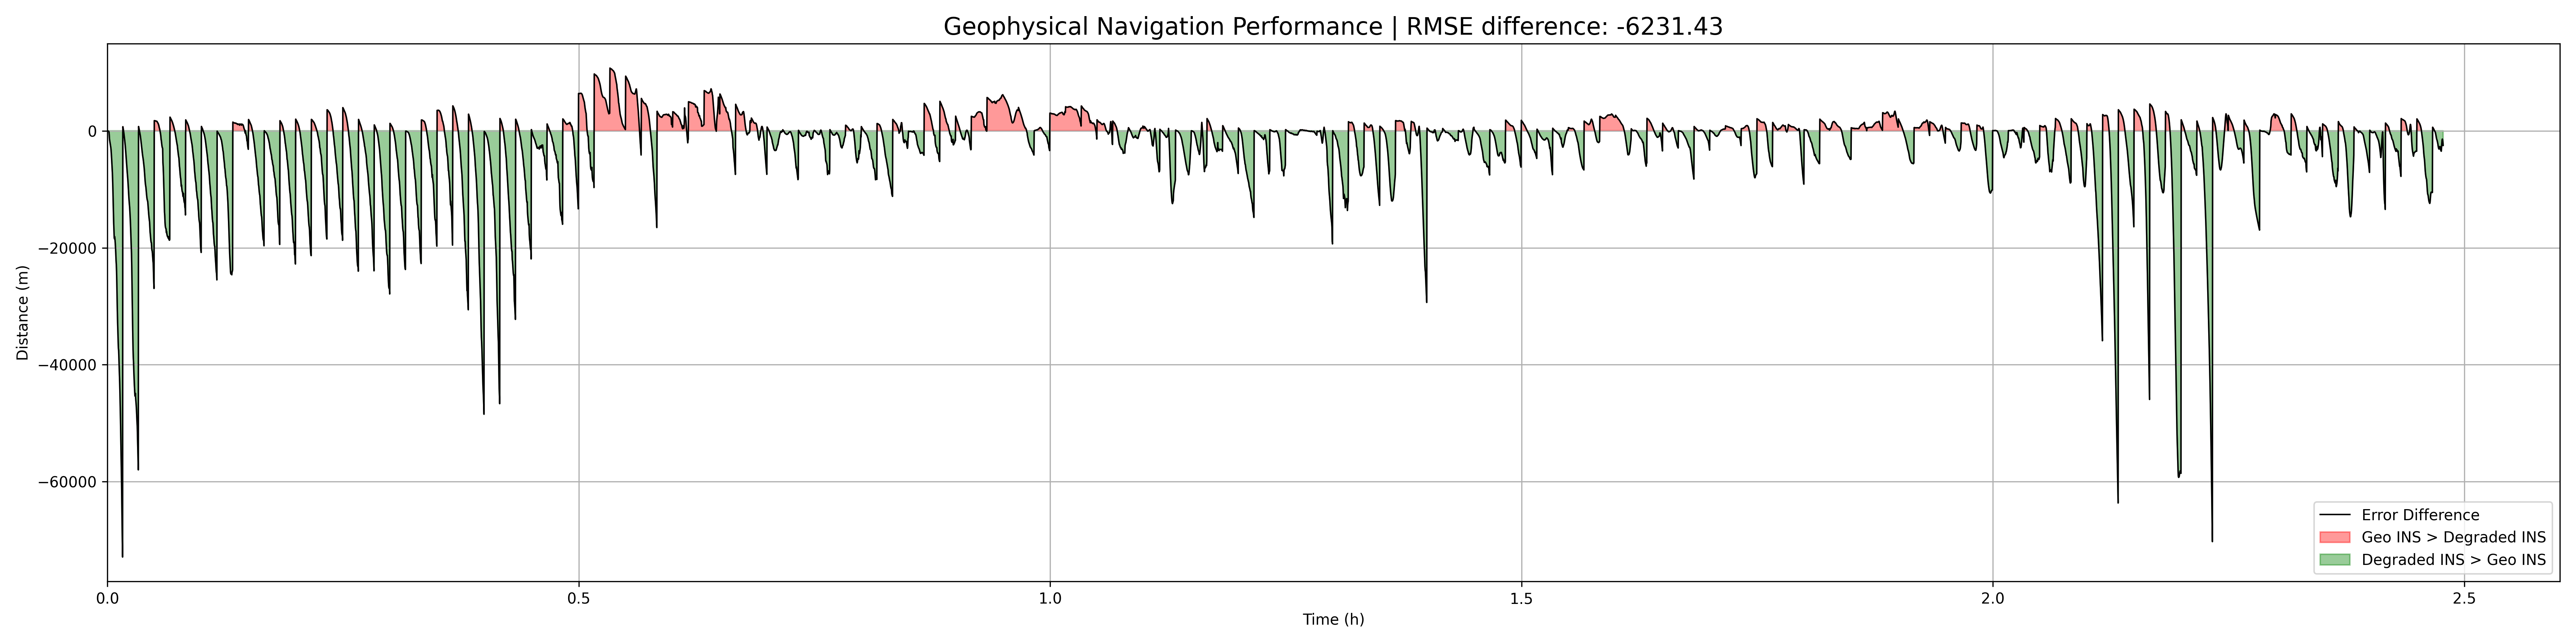
\includegraphics[width=\textwidth]{figures/good/2023-08-06_14-48-05_grav.png}
    \caption{Geo-RBPF with Gravity aiding vs INS; 6231\,m RMSE improvement over INS baseline.}
\end{figure}
\end{frame}
%-----------------------------------------------------
\begin{frame}{Example: Strong Performance} 
    \begin{figure}[b]
        \centering
        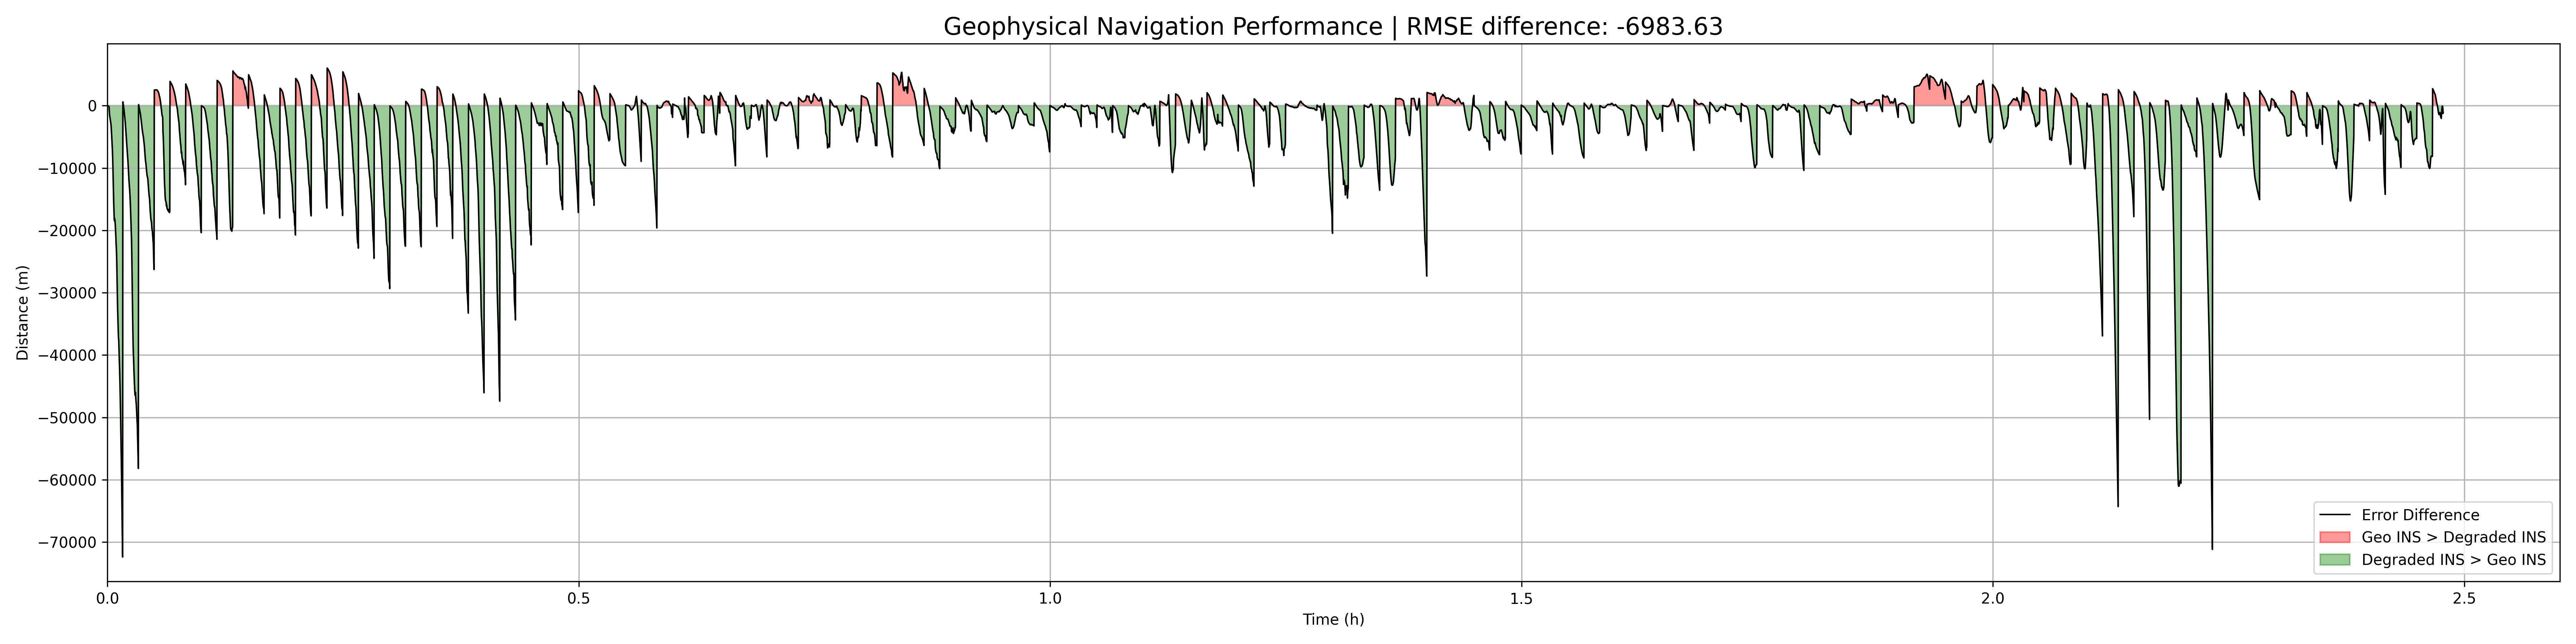
\includegraphics[width=\textwidth]{figures/good/2023-08-06_14-48-05_combined.png}
        \caption{Geo-RBPF with Combined aiding vs INS; 6664\,m RMSE improvement over INS baseline.}
    \end{figure}
\end{frame}

%-----------------------------------------------------
\begin{frame}{Example: Weak Performance}
    \begin{figure}
        \centering
        \begin{subfigure}[b]{0.32\textwidth}
            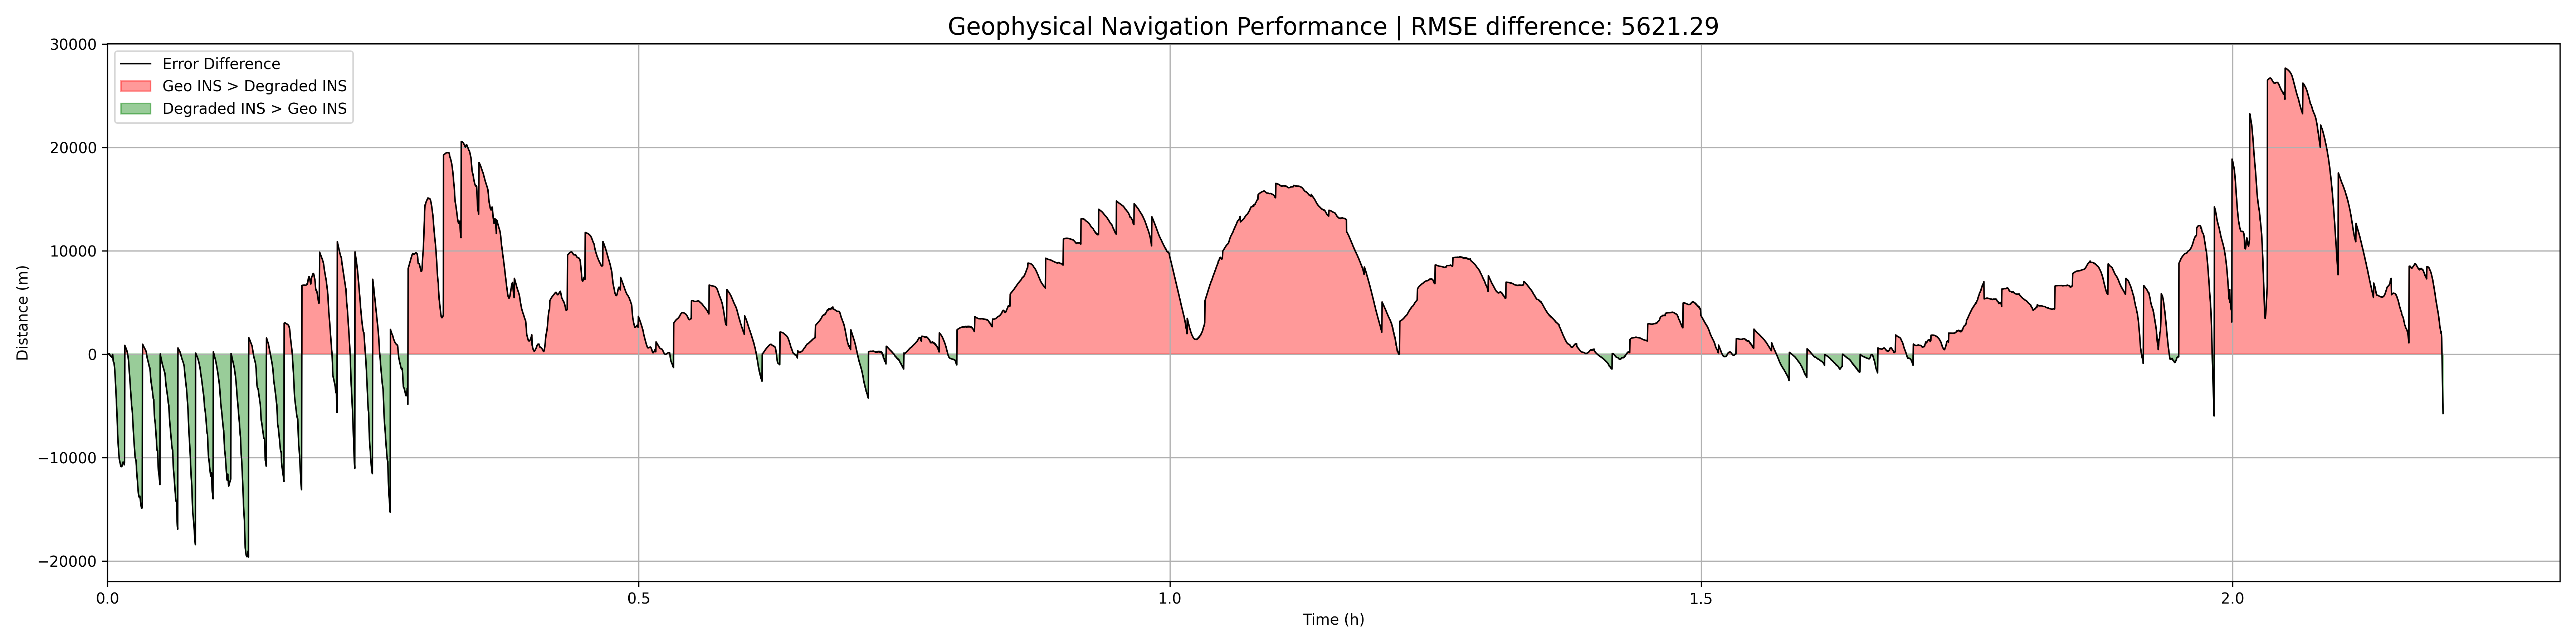
\includegraphics[width=\textwidth]{figures/poor/2025-06-18_16-52-32_mag.png}
            \caption{Magnetic aiding}
        \end{subfigure}
        \hfill
        \begin{subfigure}[b]{0.32\textwidth}
            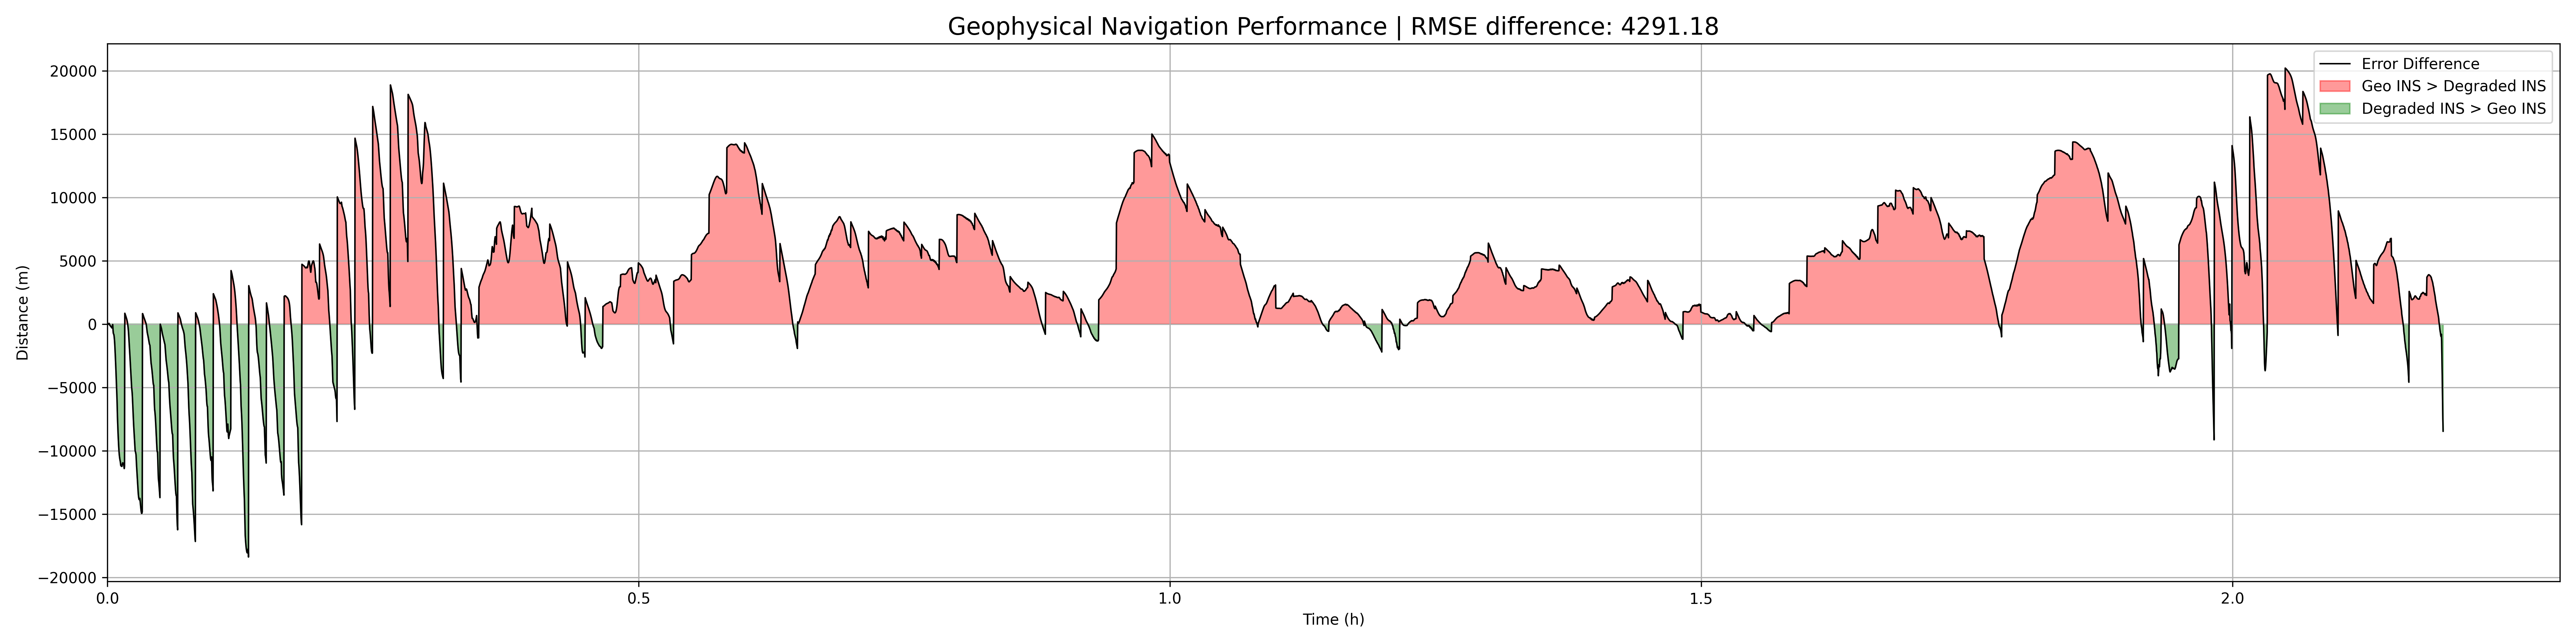
\includegraphics[width=\textwidth]{figures/poor/2025-06-18_16-52-32_grav.png}
            \caption{Gravity aiding}
        \end{subfigure}
        \hfill
        \begin{subfigure}[b]{0.32\textwidth}
            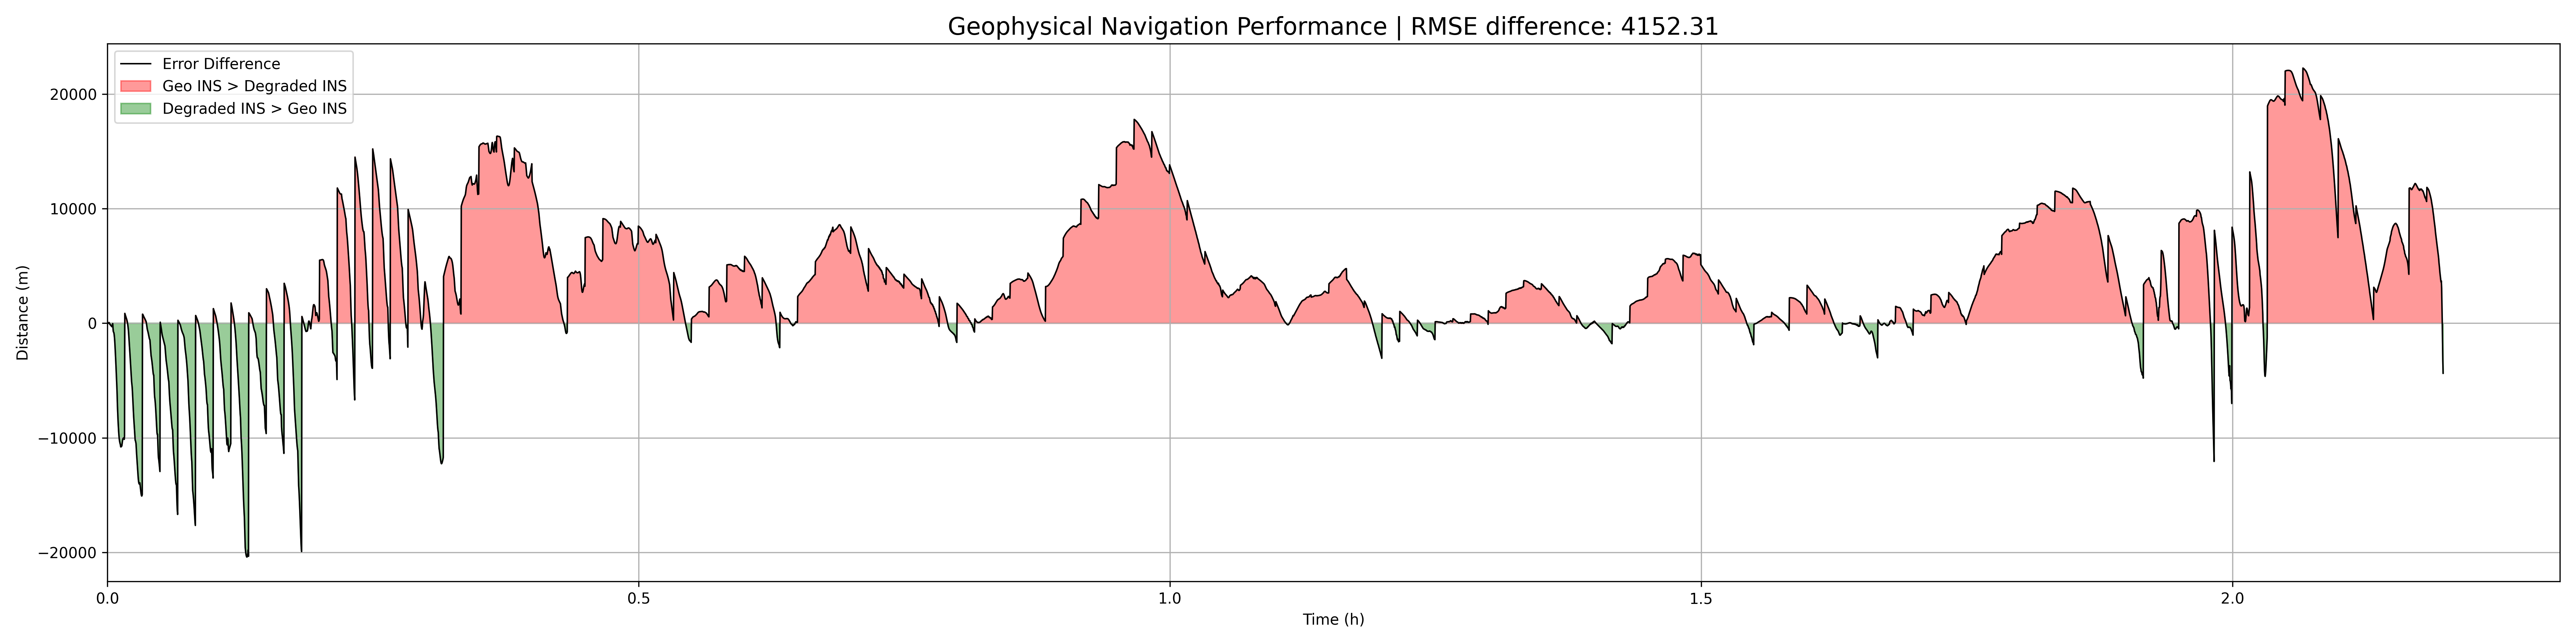
\includegraphics[width=\textwidth]{figures/poor/2025-06-18_16-52-32_combined.png}
            \caption{Combined aiding}
        \end{subfigure}
        \caption{Trajectory 2025-06-18: minimal improvement over UKF baseline. Performance is dependent on favorable anomaly field characteristics along the trajectory.}
    \end{figure}
    \begin{block}{}
        \small
        Geophysical aiding efficacy depends on anomaly field variability, trajectory geometry, and sensor noise---not all regions offer strong observability.
    \end{block}
\end{frame}

%-----------------------------------------------------
\begin{frame}{Example: Synergy from Combined Aiding}
    \begin{figure}
        \centering
        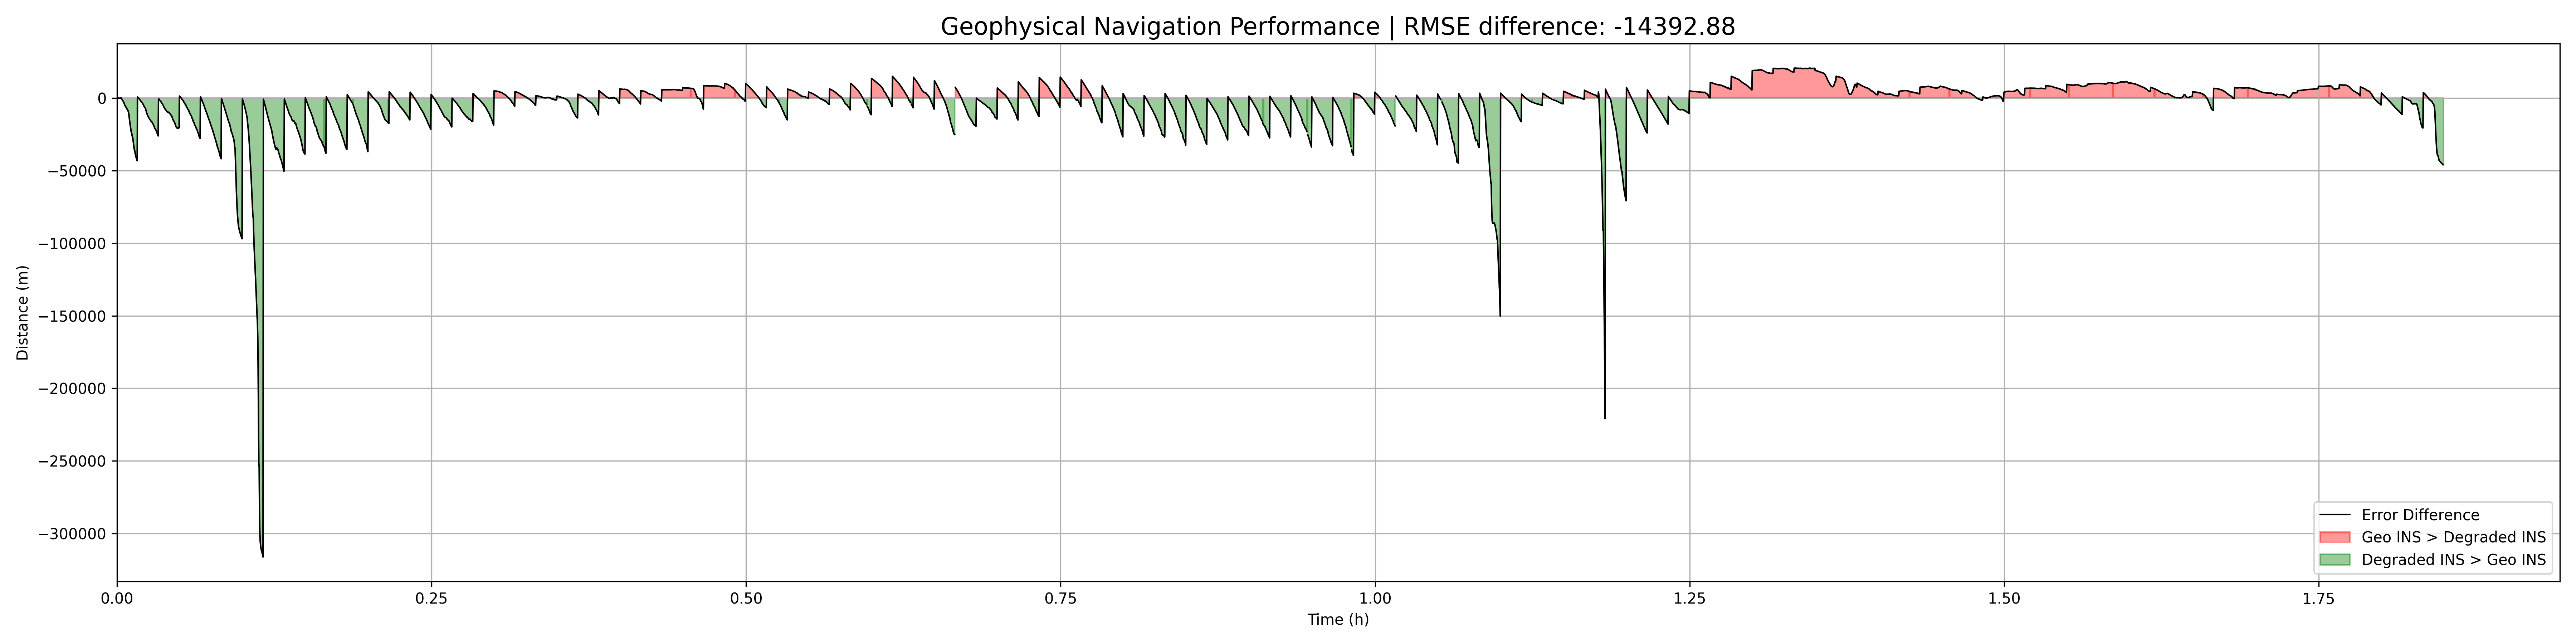
\includegraphics[width=\textwidth]{figures/mutual/2025-07-08_14-12-53_mag.png}
        \caption{Trajectory 2025-07-08: Magnetic anomaly aiding only. Strong improvement from hour 1 to 1.25.}
    \end{figure}
\end{frame}

%-----------------------------------------------------
\begin{frame}{Example: Synergy from Combined Aiding}
    \begin{figure}
        \centering
        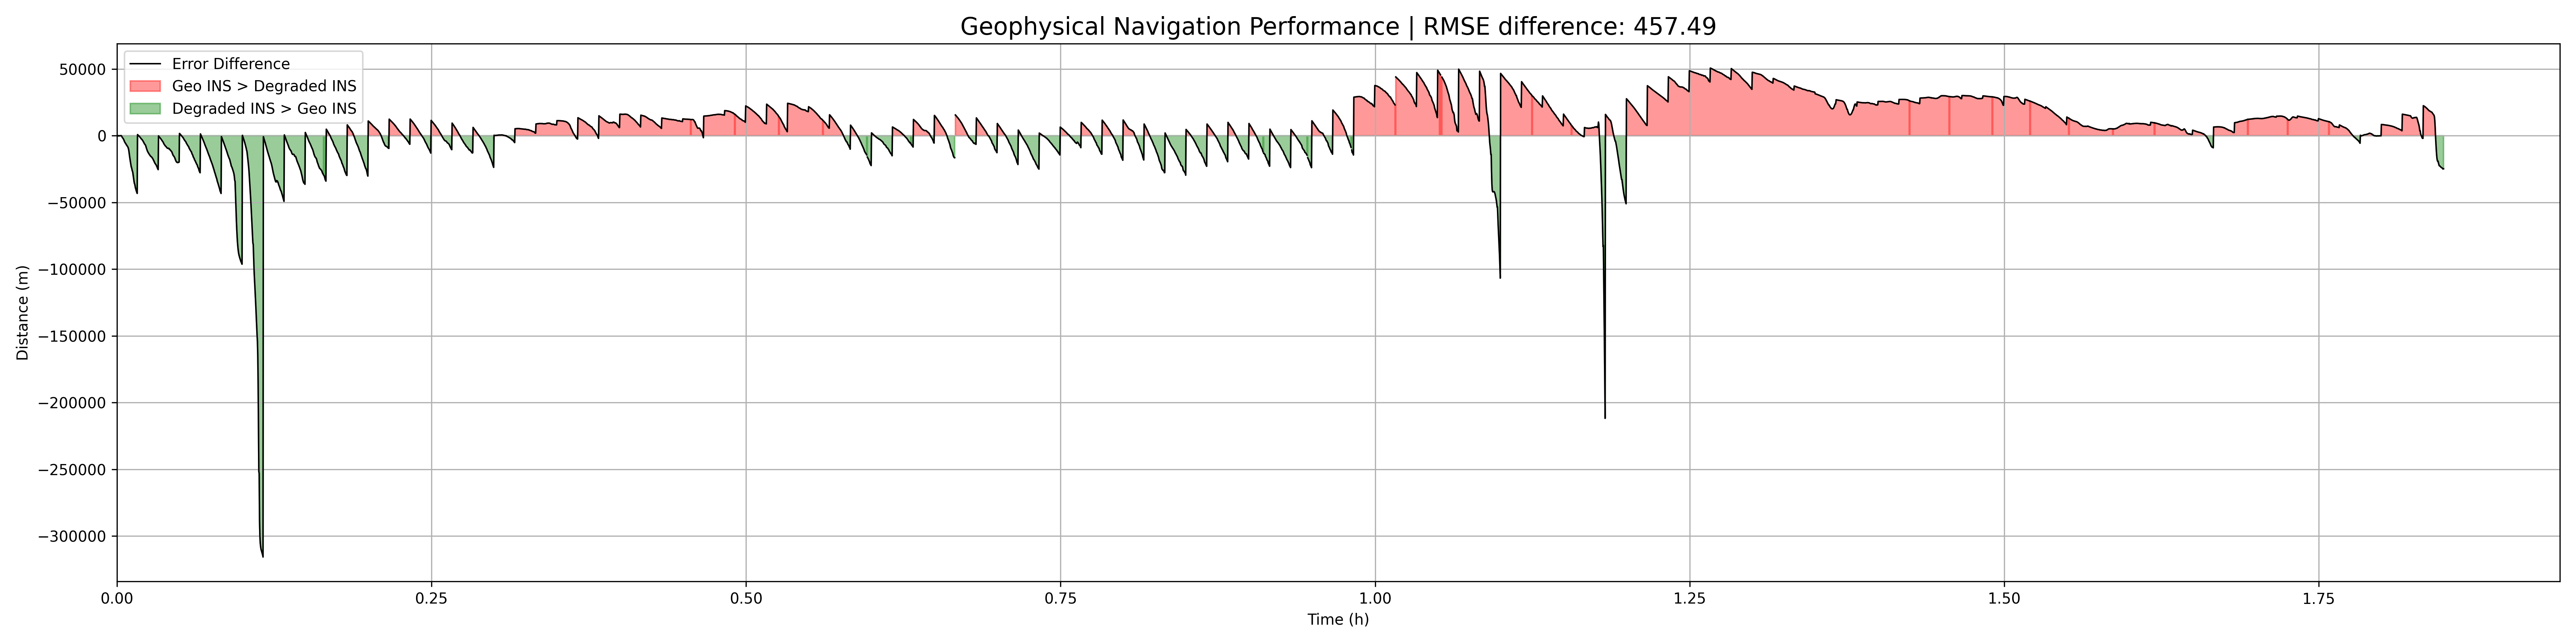
\includegraphics[width=\textwidth]{figures/mutual/2025-07-08_14-12-53_grav.png}
        \caption{Trajectory 2025-07-08: Gravity anomaly aiding only. Degraded performance from hour 1 to 1.25. Overall performance worse than UKF baseline.}
    \end{figure}
\end{frame}

%-----------------------------------------------------
\begin{frame}{Example: Synergy from Combined Aiding}
    \begin{figure}
        \centering
        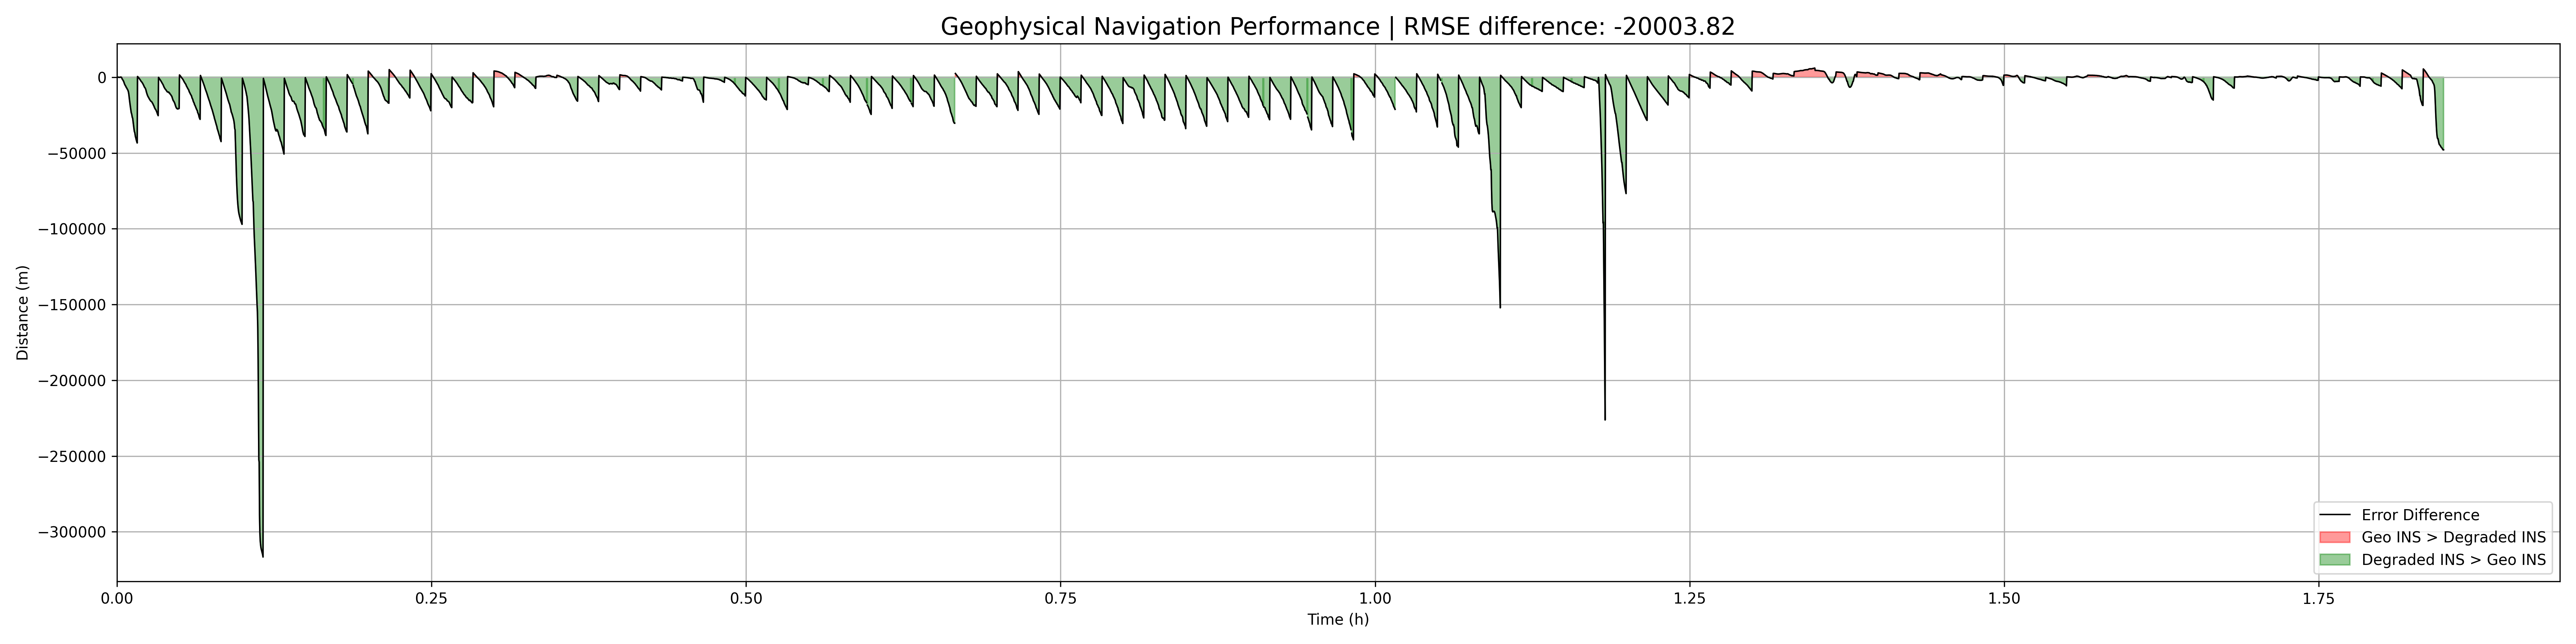
\includegraphics[width=\textwidth]{figures/mutual/2025-07-08_14-12-53_combined.png}
        \caption{Trajectory 2025-07-08: Combined gravity and magnetic anomaly aiding yields substantial improvement. Gravity and magnetic anomalies resolve ambiguities that neither can address alone.}
    \end{figure}
    \begin{exampleblock}{}
        \small
        The RBPF's particle representation enables genuine fusion of multiple non-Gaussian aiding sources---a key advantage over single-Gaussian filter architectures.
    \end{exampleblock}
\end{frame}

%%%%%%%%%%%%%%%%%%%%%%%%%%%%%%%%%%%%%%%%%%%%%%%%%%%%%
\section{Conclusion \& Future Work}

\begin{frame}{Conclusions}
    \begin{columns}
        \begin{column}{0.55\textwidth}
            \textbf{Main findings:}
            \begin{enumerate}
                \item \textbf{Geophysical aiding works}: Mean RMSE reduction of $\sim$1,562\,km vs.\ GNSS-only RBPF baseline across all 21 trajectories
                \item \textbf{Architecture matters modestly}: RBPF provides incremental 0.2--1.4\,km RMSE improvement vs.\ UKF, with combined aiding showing the greatest benefit
                \item \textbf{Synergistic fusion}: Simultaneous gravity + magnetic aiding can resolve ambiguities neither source can handle alone
                \item \textbf{Trajectory-dependent}: Performance relies on favorable anomaly field characteristics; not all regions provide strong observability
            \end{enumerate}
        \end{column}
        \begin{column}{0.42\textwidth}
            \begin{block}{Key Takeaway}
                The RBPF is a viable architecture for performant geophysical navigation. It handles non-Gaussian posteriors from map-matching without the $O(N^{16})$ cost of a full particle filter---but the primary driver of accuracy remains the \textbf{information content} of the anomaly measurement, and \textbf{IMU quality}, not the filter alone.
            \end{block}
        \end{column}
    \end{columns}
\end{frame}

%-----------------------------------------------------
\begin{frame}{Limitations}
    Simple Gaussian measurement model ignores:
        \begin{itemize}
            \item Directional dependence of scalar magnetometer
            \item Altitude corrections, temporal variation
            \item Platform magnetic signature (hard and soft iron compensation)
        \end{itemize}
    \vspace{1em}
    Weighted-mean state estimate can lie between particle clusters in multimodal cases.\\
    \vspace{1em}
    Performance is field-dependent with no online observability estimate.\\
    \vspace{1em}
    \textbf{MEMS sensor quality} is a fundamental limit; severe degradation can overwhelm the filter's ability to extract signal from noise. Consumer MEMS-grade performance represents a lower bound; higher-quality MEMS (e.g., automotive-grade) should yield better results.
\end{frame}
%-----------------------------------------------------
\begin{frame}{Future Work}
\begin{enumerate}
    \item \textbf{Physics-informed models}: Canciani airborne magnetic navigation model accounting for vector-scalar relationships and platform signatures
    \item \textbf{Multi-modal state estimation}: K-means, GMM, or DBSCAN clustering to handle distinct particle clusters before forming navigation solution
    \item \textbf{Integrity monitoring}: Online observability metrics to identify when geophysical aiding is trustworthy
    \item \textbf{Adaptive particles}: Concentrate particles where uncertainty is highest
\end{enumerate}
\end{frame}
%-----------------------------------------------------
\begin{frame}{Summary}
    \begin{center}
        \Large
        \textbf{Geophysical anomaly navigation with MEMS-grade sensors using a Rao-Blackwellized Particle Filter produces a meaningful reduction in drift error.}
    \end{center}
    \vspace{1em}
    \begin{center}
        \Large \textbf{Thank you! Questions?}
    \end{center}
    \vspace{1em}
    \begin{center}
        \small
        James Brodovsky\\
        Ph.D Candidate, Temple University\\
        jbrodovsky@temple.edu \\
        \vspace{.5em}
        \url{https://jbrodovsky.github.io} \\
        \url{https://github.com/jbrodovsky/strapdown-rs}
    \end{center}
\end{frame}

%%%%%%%%%%%%%%%%%%%%%%%%%%%%%%%%%%%%%%%%%%%%%%%%%%%%%
\appendix

\begin{frame}{Backup: Full State Vector}
    \textbf{Extended state vector for geophysically-aided RBPF:}
    \[
    \mathbf{x} = \left[\begin{array}{cccccccccccccccc}
      L & \lambda & h & v_n & v_e & v_d & \phi & \theta & \psi & b_{a_x} & b_{a_y} & b_{a_z} & b_{g_x} & b_{g_y} & b_{g_z} & \mathbf{b}_{\text{geo}}^\top
    \end{array}\right]^\top
    \]
    \begin{itemize}
        \item 16 states for single-anomaly aiding (gravity or magnetic)
        \item 17 states for dual-anomaly aiding (both)
        \item Nonlinear partition: $(L, \lambda)$ --- handled by particles
        \item Linear partition: all remaining 14--15 states --- handled by Kalman filter per particle
    \end{itemize}
\end{frame}

\begin{frame}{Backup: Strapdown Mechanization}
    \textbf{Attitude update (Z-Y-X Euler, body to nav frame):}
    \[
    \mathbf{C}_{t+1} \approx \mathbf{C}_t \left( I + \boldsymbol{\Omega}_{b} \Delta t \right) - \left( \boldsymbol{\Omega}_{i} + \boldsymbol{\Omega}_{n} \right) \mathbf{C}_t \Delta t
    \]

    \textbf{Velocity update:}
    \[
    \mathbf{v}_{t+1} \approx \mathbf{v}_{t} + \left( \hat{\mathbf{f}}_{t} + \mathbf{g}_t - \left( 2\boldsymbol{\Omega}_{i} + \boldsymbol{\Omega}_{n} \right) \mathbf{v}_t \right) \Delta t
    \]

    \textbf{Position update (WGS-84):}
    \[
    L_{t+1} = L_{t} + \frac{1}{2} \left( \frac{v_{n,t}}{R_n(L_t)+h_t} + \frac{v_{n,t+1}}{R_n(L_{t+1})+h_{t+1}} \right) \Delta t
    \]
    \[
    \lambda_{t+1} = \lambda_t + \frac{1}{2}\left(\frac{v_{e,t}}{(R_e(L_t)+h_t)\cos L_t} + \frac{v_{e,t+1}}{(R_e(L_{t+1})+h_{t+1})\cos L_{t+1}}\right)\Delta t
    \]

    Reference: Groves, \emph{Principles of GNSS, Inertial, and Multisensor Integrated Navigation Systems}, 2nd ed., Ch.\ 5.3--5.5
\end{frame}

\end{document}
